\section{Ejercicio 3}
\subsection{Introducción}

En este ejercicio se implementará la siguiente máquina de Moore provista por la cátedra mediante su diagrama de estados(\ref{Diagrama_de_estados_Ej3}):

\begin{figure}[H]
\begin{center}
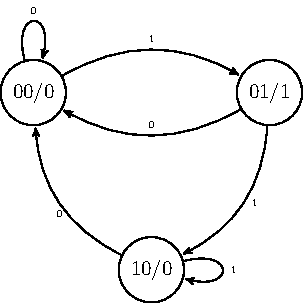
\includegraphics[scale=0.75]{Ejercicio3/Diagramas/TransicionesEj3}
\caption{Diagrama de estados}
\end{center}
\label{Diagrama_de_estados_Ej3}
\end{figure}

Esta máquina cuenta con tres estados que son los siguientes:

\begin{table}[H]
	\begin{center}
	\scalebox{0.8}{
		\begin{tabular}{c|c|c}
		Estado & $Q_1$                  & $Q_0$ \\ \hline
		A      & \multicolumn{1}{c|}{0} & 0     \\
		B      & \multicolumn{1}{c|}{0} & 1     \\
		C      & \multicolumn{1}{c|}{1} & 0     \\
		\end{tabular}
	}
	\caption{Estados utilizados}
	\end{center}
	\label{Estados_Ej3}
\end{table}

La tabla de transición para esta máquina es la que se muestra a continuación:

\begin{table}[H]
\begin{center}
\scalebox{0.8}{
\begin{tabular}{c|cc|c}
\multirow{2}{*}{Estado Actual} & \multicolumn{2}{c|}{Entrada} & Salida \\
                               & X=0                    & X=1 & S      \\ \hline
A                              & \multicolumn{1}{c|}{A} & B   & 0      \\
B                              & \multicolumn{1}{c|}{A} & C   & 1      \\
C                              & \multicolumn{1}{c|}{A} & C   & 0     
\end{tabular}
}
\label{Tabla_de_transiciones_Ej3}
\caption{Tabla de transiciones}
\end{center}
\end{table}


%Mapas de Karnaugh 
\subsection{Implementación}

Se necesitan dos bits para almacenar los tres estados utilizados, por lo que se necesitarán dos Flip-Flop D para guardarlos en memoria.
Desarrollando las tablas obtenemos los siguientes mapas de Karnaugh que nos indicarán los circuitos lógicos necesarios.

\begin{center}
	\hspace*{\fill}
   \begin{tikzpicture}[x=8mm,y=8mm]
    \K[x bits = 2, y bits = 1, label={$D_1$},
       variable names = {$Q_0$,$X$,$Q_1$,}]
    { 
      000,0,    
      001,0,   
      010,0,   
      011,1,       
      100,0, 
      101,X,
      110,1,
 	  111,X,

    }
    \newcommand*{\myKG}[4][0.1]{\KG[x bits = 2,y bits = 1,group opacity = #1,
                  #2]{#3}{#4}}
    \myKG     {group color = red,  group distance=0.35}{011}{111}
    \myKG     {group color = pink,  group distance=0.35}{111}{110}



    %=====================================================================
    % in picture comments
    %=====================================================================

    \path (1,-1.5) node[anchor = north, align = left] (eq1){%
    $D_1 = 
       \ul{red}{${Q_0X}\,$}
       +\ul{pink}{${Q_1X}\,$}  
    $};
    
  \end{tikzpicture}
	\hspace{2mm}
   \begin{tikzpicture}[x=8mm,y=8mm]
   
\K[x bits = 2, y bits = 1, label={$D_0$},
       variable names = {$Q_0$,$X$,$Q_1$,}]
    { 
      000,0,    
      001,1,   
      010,0,   
      011,0,       
      100,0, 
      101,0,
      110,X,
 	  111,X,

    }
    \newcommand*{\myKG}[4][0.1]{\KG[x bits = 2,y bits = 1,group opacity = #1,
                  #2]{#3}{#4}}
    \myKG     {group color = red,  group distance=0.35}{001}{001}




    %=====================================================================
    % in picture comments
    %=====================================================================

    \path (1,-1.5) node[anchor = north, align = left] (eq1){%
    $D_0 = 
       \ul{red}{$\ol{Q_1Q_0}\,{X}\,$}
    $};
    
  \end{tikzpicture}
	\hspace{2mm}
	\hspace*{\fill}
\end{center}
Dando como resultado el siguiente circuito:
 \begin{figure}[H]
\begin{center}
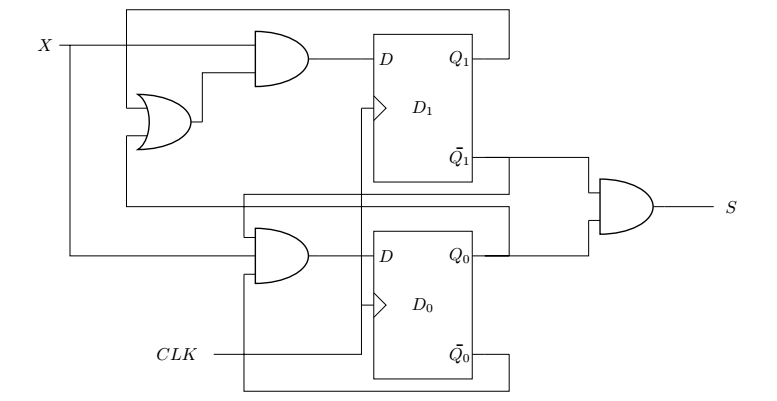
\includegraphics[scale=0.5]{Ejercicio3/Circuitos/LogicaEj3}
\caption{Lógica de entrada}
\end{center}
\label{Logica_de_entrada_Ej3}
\end{figure}

Por otro lado, se puede observar claramente en la tabla de transiciones (\ref{Tabla_de_transiciones_Ej3}) que el valor de la salida sólo se encuentra alto para el caso del estado B. Dando como resultado que el valor de la salida va a estar dado por:
\begin{equation}
S=\bar{Q_1}Q_0
\end{equation}
Por ende, la lógica de salida para nuestra máquina de estados estará representada por:
 \begin{figure}[H]
\begin{center}
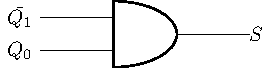
\includegraphics[scale=0.75]{Ejercicio3/Circuitos/SalidaEj3}
\caption{Lógica de salida}
\end{center}
\label{Logica_de_salida_Ej3}
\end{figure}

Se adjunta simulación en Proteus para respaldar el diseño.

\subsection{Consideraciones para la placa}
La cátedra solicita que las entradas y salidas de la máquina de estados tengan una lógica de 5V mientras que la lógica interna sea de $3.3\,V$. \par 
Como primer medida, se utilizará un regulador de tensión($LMS1587CS$) para obtener la tensión para la lógica interna.
Dentro del circuito interno no se podrán usar integrados de puertas discretas usuales sino que será necesario utilizar integrados de baja tensión, en nuestro caso un integrado ($74AUP1G08-Q1$) para las compuertas AND de dos entradas y un ($74AUP2G32$) para la compuerta OR. Por otro lado, también será necesario un Flip Flop D de baja tensión ($74AUP1G79$). \par


\subsubsection{Uso de level shifters}
Para variar la tensión de entrada de $5\,V$ a $3.3\,V$ se utilizan dos transistores NPN a modo de level shifter como se muestran en la figura (\ref{33to5v}).

 \begin{figure}[H]
\begin{center}
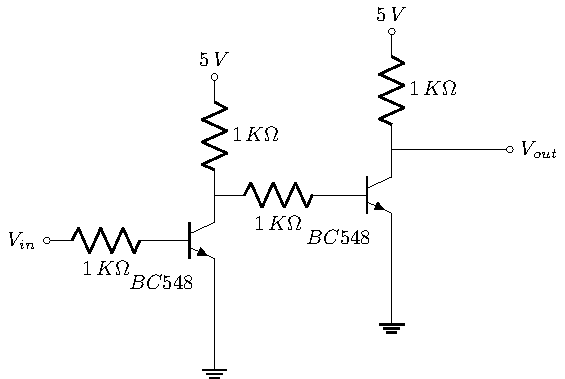
\includegraphics[scale=0.75]{Ejercicio3/Circuitos/3_3Vto5V}
\caption{Level Shifter 3.3V to 5V}
\end{center}
\label{33to5v}
\end{figure}
Para variar la tensión de entrada de $3.3\,V$ a $5\,V$ se utilizan dos transistores NPN a modo de level shifter como se muestran en la figura (\ref{5vto33v}).

 \begin{figure}[H]
\begin{center}
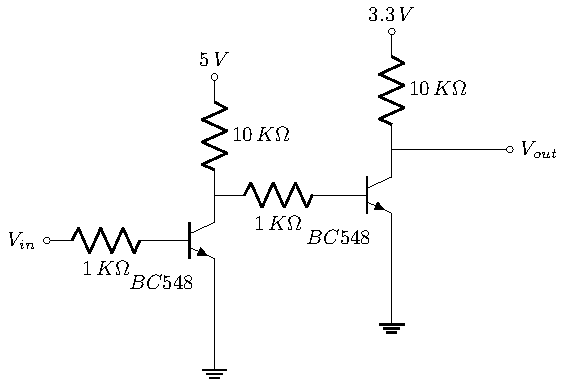
\includegraphics[scale=0.75]{Ejercicio3/Circuitos/5Vto3_3V}
\caption{Level Shifter 5V to 3.3V}
\end{center}
\label{5vto33v}
\end{figure}

\subsubsection{Componenetes utilizados}
\begin{itemize}
\item Regulador de tensión 5V a 3.3V - $LMS1587CS$
\item Flip-Flop D - $74AUP1G79$
\item Compuerta AND 2 entradas - $74AUP1G08-Q1$
\item Compuerta OR 2 entradas - $74AUP2G32$
\item Transistor NPN BC548 - $74AUP2G32$
\end{itemize}





